\documentclass[11pt,a4paper]{article}

% ---------- packages ----------
\usepackage[utf8]{inputenc}
\usepackage[T1]{fontenc}
\usepackage{lmodern}
\usepackage[a4paper,margin=1in,headheight=14pt]{geometry}
\usepackage{graphicx}
\usepackage{xcolor}
\usepackage[most]{tcolorbox}
\usepackage{listings}
\usepackage{booktabs}
\usepackage{array}
\usepackage{enumitem}
\usepackage{titlesec}
\usepackage{caption}
\usepackage{fancyhdr}
\usepackage{tikz}
\usepackage{amssymb}
\usepackage{microtype}
\usetikzlibrary{arrows.meta,positioning,shapes.geometric,calc,backgrounds,fit}
\usepackage[colorlinks=true,linkcolor=buetred,urlcolor=urlteal,citecolor=buetred]{hyperref}

% ---------- colors ----------
\definecolor{buetred}{HTML}{9E1B22}
\definecolor{navy}{HTML}{0B2545}
\definecolor{deepblue}{HTML}{13315C}
\definecolor{orange}{HTML}{E8871E}
\definecolor{green}{HTML}{2E7D32}
\definecolor{urlteal}{HTML}{0E7C7B}
\definecolor{termbg}{HTML}{10131A}
\definecolor{termfg}{HTML}{D7DCE3}
\definecolor{lightgray}{HTML}{F4F5F8}
\definecolor{rulegray}{HTML}{C9CED8}

% ---------- section styling ----------
\titleformat{\section}{\Large\bfseries\color{navy}}{\thesection}{0.6em}{}[{\color{orange}\titlerule[1.5pt]}]
\titleformat{\subsection}{\large\bfseries\color{deepblue}}{\thesubsection}{0.6em}{}
\titleformat{\subsubsection}{\normalsize\bfseries\color{deepblue}}{\thesubsubsection}{0.6em}{}
\titlespacing*{\section}{0pt}{16pt}{8pt}

% ---------- headers/footers ----------
\pagestyle{fancy}
\fancyhf{}
\renewcommand{\headrulewidth}{0.4pt}
\fancyhead[L]{\small\color{navy}Optimistic TCP ACK Attack}
\fancyhead[R]{\small\color{navy}CSE406 \textbullet\ Group 10}
\fancyfoot[C]{\small\thepage}

% ---------- terminal listing style ----------
\lstdefinestyle{term}{
  basicstyle=\ttfamily\scriptsize\color{termfg},
  backgroundcolor=\color{termbg},
  breaklines=true, breakatwhitespace=false,
  columns=fullflexible, keepspaces=true,
  frame=single, rulecolor=\color{termbg}, framexleftmargin=4pt,
  xleftmargin=6pt, xrightmargin=6pt, aboveskip=8pt, belowskip=4pt,
  literate={→}{{$\rightarrow$}}1 {≥}{{$\geq$}}1 {×}{{$\times$}}1 {—}{{-}}1
}
\lstdefinestyle{codebox}{
  basicstyle=\ttfamily\footnotesize,
  backgroundcolor=\color{lightgray},
  breaklines=true, columns=fullflexible,
  frame=single, rulecolor=\color{rulegray},
  xleftmargin=6pt, xrightmargin=6pt, aboveskip=8pt, belowskip=4pt,
}

% ---------- callout box ----------
\newtcolorbox{keybox}[1][Key Result]{
  enhanced, breakable, colback=green!5, colframe=green!70!black,
  boxrule=0.8pt, arc=2pt, left=8pt, right=8pt, top=6pt, bottom=6pt,
  fonttitle=\bfseries, coltitle=white, colbacktitle=green!60!black, title={#1}}
\newtcolorbox{notebox}[1][Note]{
  enhanced, breakable, colback=orange!6, colframe=orange!80!black,
  boxrule=0.8pt, arc=2pt, left=8pt, right=8pt, top=6pt, bottom=6pt,
  fonttitle=\bfseries, coltitle=white, colbacktitle=orange!85!black, title={#1}}

\captionsetup{font=small,labelfont={bf,color=navy}}
\setlist{itemsep=2pt,topsep=3pt}

\begin{document}

% ============================ COVER PAGE ============================
\begin{titlepage}
\centering
\vspace*{0.3cm}
{\color{navy}\rule{\textwidth}{2pt}}\\[0.15cm]
{\large\bfseries\color{navy} BANGLADESH UNIVERSITY OF ENGINEERING AND TECHNOLOGY}\\[0.15cm]
{\normalsize\color{deepblue} Department of Computer Science and Engineering}\\[0.1cm]
{\color{navy}\rule{\textwidth}{2pt}}\\[0.7cm]


\includegraphics[width=0.30\textwidth]{figures/buet_logo.png}\\[0.7cm]

{\large\color{deepblue} CSE 406 --- Computer Security Sessional}\\[0.3cm]
{\normalsize Final Report \& Implementation Demonstration}\\[0.9cm]

{\color{buetred}\rule{0.8\textwidth}{1.2pt}}\\[0.35cm]
{\huge\bfseries\color{navy} Optimistic TCP ACK Attack}\\[0.35cm]
{\Large\color{deepblue} Against a Streaming Server}\\[0.30cm]
{\large\itshape\color{black!70} Implementation, Analysis, and Defense in an Isolated Docker Testbed}\\[0.35cm]
{\color{buetred}\rule{0.8\textwidth}{1.2pt}}\\[1.1cm]

\begin{tabular}{@{}rl@{}}
\multicolumn{2}{c}{\large\bfseries\color{navy} Submitted by --- Group 10, Section A1}\\[0.5cm]
\large Niloy Das Robin & \large 2105019 \\[0.25cm]
\large Sayjad Rahman & \large 2105021 \\
\end{tabular}\\[1.1cm]

\begin{tabular}{@{}rl@{}}
\bfseries Supervisor: & Md Zim Mim Siddiqee Sowdha \\[0.2cm]
\bfseries Course: & CSE 406 --- Cyber Security Sessional \\[0.2cm]
\bfseries Attack (Tool \#16): & Optimistic TCP Acknowledgment \\
\end{tabular}\\[1.4cm]

{\color{navy}\rule{\textwidth}{1pt}}\\[0.15cm]
{\small\color{black!60} Submitted: \today \quad\textbullet\quad All experiments confined to a self-owned, isolated lab testbed}\\
\end{titlepage}

% ============================ ABSTRACT ============================
\thispagestyle{fancy}
\begin{tcolorbox}[colback=lightgray,colframe=navy,boxrule=1pt,arc=2pt,
  title={\bfseries Abstract},fonttitle=\color{white}\bfseries,colbacktitle=navy]
\small
We implement, demonstrate, and defend against the \textbf{optimistic TCP acknowledgment
attack} --- a specification-level flaw in which a misbehaving TCP receiver acknowledges
data it has not yet received (or never receives), tricking the sender's congestion
control into believing the path is fast and loss-free. We built a from-scratch
raw-socket attack tool in C, a custom TCP streaming ``victim'' server, and a
three-node isolated Docker testbed. Against a CUBIC server on a realistic lossy link
(20\,ms delay, 2\% loss) the attack coerced the server's congestion window from
\textbf{3 to 2{,}339 segments} ($\approx$\,780$\times$) and drove it to transmit
\textbf{1{,}677\,MB in 14 seconds}; across the Reno/CUBIC option matrix the measured
egress amplification reached \textbf{$\sim$95$\times$} over an honest client on the
identical link. We further
characterised the attack across Reno and CUBIC with and without SACK/timestamps, and
implemented a working server-side defense (Sherwood's randomly-skipped-segment test)
that detects the lie on the first probe and resets the flow, cutting the attacker's
throughput from \textbf{898 to 2.49\,Mbit/s} while leaving honest clients completely
unaffected. Every result in this report is reproduced from real measurements in our
testbed.
\end{tcolorbox}

{\small\tableofcontents}
\newpage

% ============================ 1. INTRODUCTION ============================
\section{Introduction and Objective}

TCP's congestion control silently assumes one thing about the other end of a connection:
that its acknowledgments are \emph{honest} --- that an ACK for byte $N$ means byte $N$
truly arrived. Nothing in the protocol enforces this. The \textbf{optimistic ACK attack},
first described by Savage \textit{et al.} (1999)~\cite{savage} and weaponised as a
denial-of-service amplifier by Sherwood \textit{et al.} (2005)~\cite{sherwood}, exploits
exactly this trust: a receiver that acknowledges data \emph{before it arrives} emulates a
near-zero round-trip time and zero loss, so the sender's congestion window grows without
the brake that loss would normally apply.

\textbf{Assigned tool:} Optimistic TCP Acknowledgment (Tool \#16). \textbf{Objective:}
build the attack from scratch against our own streaming server, demonstrate and quantify
its effect, analyse \emph{why} it succeeds, and design a countermeasure. This report
answers the four required questions directly:

\begin{enumerate}[label=\textbf{(\alph*)}]
  \item \textbf{Steps of the attack, snapshots, victim screen} --- Section~\ref{sec:steps}.
  \item \textbf{Is the attack successful? Why / why not?} --- Section~\ref{sec:success}.
  \item \textbf{Observed output on attacker / victim / other PCs} --- Section~\ref{sec:observed}.
  \item \textbf{Countermeasure design and how it works} --- Section~\ref{sec:defense}.
\end{enumerate}

\begin{notebox}[Ethics and scope]
Every technique here was executed \emph{exclusively} inside our own isolated Docker
network, against our own streaming server. Nothing was pointed at any host, network, or
service we do not own. The attack is a well-documented 25-year-old academic result; the
purpose of studying it is to understand \emph{why} TCP trusts its receivers and how modern
systems defend against that trust being abused.
\end{notebox}

% ============================ 2. BACKGROUND ============================
\section{Background: Why the Attack Works}

A TCP sender maintains a \textbf{congestion window} (\texttt{cwnd}) --- the amount of
unacknowledged data it dares to have in flight. In \emph{slow start} it doubles
\texttt{cwnd} each round-trip; in \emph{congestion avoidance} it grows linearly. The
\emph{only} thing that shrinks \texttt{cwnd} is a congestion signal --- a lost segment,
inferred from a timeout or duplicate ACKs. Crucially, TCP is \textbf{ACK-clocked}: new
data is released as ACKs return, so the rate at which ACKs arrive \emph{is} the sending
rate.

\begin{keybox}[The core insight]
An optimistic receiver sends a stream of acknowledgments for data the sender
\emph{has not sent yet}. To the sender this looks like: (i) every segment is being
delivered, (ii) instantly (near-zero RTT), and (iii) with zero loss. So its congestion
control does exactly what it was designed to do on a fast, clean path --- it inflates
\texttt{cwnd} and floods the link. \textbf{The sender is not malfunctioning; it is
behaving correctly on false information.}
\end{keybox}

Because a $\sim$40-byte ACK can acknowledge an entire window of data, a \emph{trickle} of
tiny upstream ACKs coerces a \emph{torrent} of downstream data. When the victim is a
streaming server, its own uplink becomes the weapon --- the amplification structure of a
reflection DoS, but the amplifier is the victim's own correctly-functioning TCP stack.

% ============================ 3. TESTBED ============================
\section{Testbed Architecture}
\label{sec:testbed}

The entire project runs in Docker Compose --- three network nodes on an isolated bridge
network \texttt{labnet} (\texttt{172.28.0.0/16}), plus a control dashboard. Nothing is
installed on the host; if it is not in the Compose file, it does not count as working.

\begin{figure}[h]
\centering
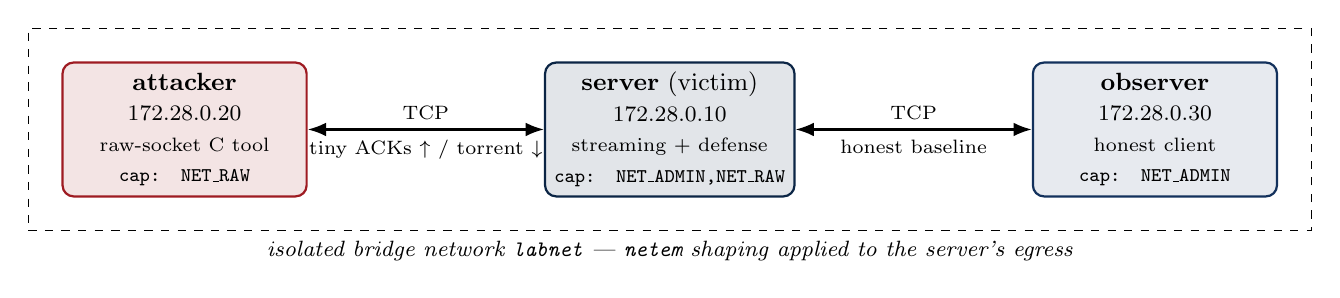
\begin{tikzpicture}[
  node distance=2.6cm and 3.0cm, font=\small,
  box/.style={draw,thick,rounded corners,minimum width=3.1cm,minimum height=1.7cm,align=center},
  att/.style={box,fill=buetred!12,draw=buetred},
  srv/.style={box,fill=navy!12,draw=navy},
  obs/.style={box,fill=deepblue!10,draw=deepblue},
  >=Latex]
\node[att] (a) {\textbf{attacker}\\\footnotesize 172.28.0.20\\\scriptsize raw-socket C tool\\\scriptsize \texttt{cap: NET\_RAW}};
\node[srv,right=of a] (s) {\textbf{server} (victim)\\\footnotesize 172.28.0.10\\\scriptsize streaming + defense\\\scriptsize \texttt{cap: NET\_ADMIN,NET\_RAW}};
\node[obs,right=of s] (o) {\textbf{observer}\\\footnotesize 172.28.0.30\\\scriptsize honest client\\\scriptsize \texttt{cap: NET\_ADMIN}};
\draw[<->,thick] (a) -- node[above,font=\scriptsize]{TCP} node[below,font=\scriptsize]{tiny ACKs $\uparrow$ / torrent $\downarrow$} (s);
\draw[<->,thick] (s) -- node[above,font=\scriptsize]{TCP} node[below,font=\scriptsize]{honest baseline} (o);
\node[draw,dashed,fit=(a)(s)(o),inner sep=12pt,label={[font=\footnotesize\itshape]below:isolated bridge network \texttt{labnet} --- \texttt{netem} shaping applied to the server's egress}] {};
\end{tikzpicture}
\caption{Three-node isolated testbed. The \texttt{server} is the bulk sender in every
scenario, so the \texttt{netem} bottleneck (20\,ms delay, 2\% loss) is applied to
\emph{its} egress. A fourth container (\texttt{dashboard}) drives and visualises the
others through the Docker socket.}
\label{fig:topology}
\end{figure}

\begin{table}[h]
\centering\small
\begin{tabular}{@{}p{4.2cm} p{3.3cm} p{6.4cm}@{}}
\toprule
\textbf{Component} & \textbf{Role} & \textbf{Implementation} \\
\midrule
\texttt{server/stream\_server.c} & Victim streaming server & C, per-socket CC via \texttt{setsockopt(TCP\_CONGESTION)} \\
\texttt{server/defense\_server.c} & Defended server & C raw-socket, skip-test detector \\
\texttt{attacker/optack.c} & Attack tool & C raw sockets, hand-built IP/TCP + checksums \\
\texttt{attacker/optack\_proto.py} & Prototype & Scapy, packet-format validation \\
\texttt{scripts/*.sh}, \texttt{sweep.py} & Test harness & Gates, shaping, multi-CC sweep \\
\texttt{dashboard/} & Live control panel & Python stdlib + HTML/JS, one-command \\
\bottomrule
\end{tabular}
\caption{Testbed components. The traffic-shaping realism (\texttt{tc netem}) was verified
directly: configured 20\,ms delay measured as 20--23\,ms RTT, configured 2\% loss measured
as 2.6\% over 500 probes, and the 10\,Mbit rate cap measured at 9.43\,Mbit/s.}
\end{table}

\begin{notebox}[Design decision: no kernel-vs-tool conflict]
The attack tool drives the \emph{entire} connection --- including the three-way
handshake --- from a raw socket (\texttt{IP\_HDRINCL}), so the host kernel never holds a
TCP control block for the 4-tuple. An \texttt{iptables} rule suppresses the kernel's own
RSTs for the flow. This is the deliberate resolution of the ``two stacks fighting over one
4-tuple'' problem, decided once and applied throughout.
\end{notebox}

% ============================ 4. ATTACK DESIGN ============================
\section{Attack Design and Implementation}
\label{sec:design}

The attack tool (\texttt{optack.c}) is a \textbf{misbehaving receiver}. After the
handshake it does not wait for data before acknowledging it; it \emph{predicts} what the
server will send and acknowledges it early, advancing the acknowledgment number ahead of
genuinely-received data. The core loop follows Sherwood's Algorithm~1: advance the ACK by
the current window estimate, send the forged ACK, and grow the window --- with
\textbf{overrun detection and recovery} (a self-tuning AIMD ``ack-ahead'' lead that halves
whenever the flow stalls, so it can never dead-lock).

Two subtleties make the attack robust against a realistic modern receiver, both
implemented and both later shown to matter (Section~\ref{sec:matrix}):

\begin{itemize}
  \item \textbf{TCP timestamps (PAWS).} Every forged ACK echoes a plausible, monotonic
        \texttt{TSecr}, or the server's PAWS check would silently drop it.
  \item \textbf{SACK.} Negotiating SACK, as any modern client does, keeps the server's
        window open even as the attacker's recovery ACKs would otherwise look like
        duplicates.
\end{itemize}

% ============================ 5. EXECUTION & RESULTS ============================
\section{Attack Execution: Steps and Snapshots}
\label{sec:steps}

This section answers requirement~\textbf{(a)}. The attack proceeds in four observable
steps; each is backed by a real capture from our testbed.

\paragraph{Step 1 --- Establish and shape.} Bring up the testbed, start the CUBIC server,
and shape its egress to a realistic lossy link:
\begin{lstlisting}[style=codebox]
docker compose up -d
docker compose exec server tc qdisc replace dev eth0 root netem delay 20ms loss 2%
\end{lstlisting}

\paragraph{Step 2 --- Honest baseline (control).} The observer pulls data as a
well-behaved client. On the victim, \texttt{ss -ti} shows CUBIC behaving correctly ---
a small window, real RTT, and real retransmissions from the 2\% loss:
\begin{lstlisting}[style=term]
$ docker compose exec server ss -tin dst observer
ESTAB  172.28.0.10:5000  172.28.0.30:60838
   cubic rtt:21.52/0.606 mss:1448 cwnd:3 ssthresh:3
   bytes_sent:42433792 retrans:0/559 send 1614870bps minrtt:20
\end{lstlisting}

\paragraph{Step 3 --- Launch the attack.} The attacker connects and begins acknowledging
data optimistically. Its own log shows the runaway --- over 1.6\,GB ``received'' in 14
seconds, far beyond what a 20\,ms/2\%-loss link could honestly deliver:
\begin{lstlisting}[style=term]
$ /work/attack --target server --port 5000 --duration 15 --sack --timestamps -v
[optack] 172.28.0.20:25879  ->  172.28.0.10:5000  (mode=optimistic, isn=55018294)
[optack] connection established (timestamps on), streaming begins
[optack] t=1.0s  recv=111.60 MB   ack-ahead=18KB   acks=1000
[optack] t=5.0s  recv=560.72 MB   ack-ahead=450KB  acks=5000
[optack] t=10.0s recv=1235.22 MB  ack-ahead=29KB   acks=10000
[optack] t=14.0s recv=1677.19 MB  ack-ahead=0KB    acks=14000
\end{lstlisting}

\paragraph{Step 4 --- The victim's screen.} On the victim, the same \texttt{ss -ti} now
shows the signature of the attack: the congestion window has exploded and the measured
minimum RTT has collapsed toward zero:
\begin{lstlisting}[style=term]
$ docker compose exec server ss -tin dst attacker
ESTAB  172.28.0.10:5000  172.28.0.20:25879
   cubic rtt:12.157/2.983 mss:1448 cwnd:2339 ssthresh:2109
   bytes_sent:577482120 send 2228755121bps minrtt:0.89
\end{lstlisting}

A packet capture on the victim confirms the mechanism --- a dense stream of tiny,
zero-length pure ACKs arriving from the attacker (the ``trickle up'' that coerces the
``torrent down''):
\begin{lstlisting}[style=term]
$ tcpdump -i eth0 -n 'tcp and src host 172.28.0.20'
172.28.0.20.25879 > 172.28.0.10.5000: Flags [.], ack ..., win 65535, length 0
172.28.0.20.25879 > 172.28.0.10.5000: Flags [.], ack ..., win 65535, length 0
... (thousands of 0-byte ACKs per second) ...
\end{lstlisting}

\section{Was the Attack Successful? Analysis}
\label{sec:success}

This section answers requirement~\textbf{(b)}. \textbf{Yes --- the attack was
unambiguously successful.} Placing the honest control and the attack side by side on the
\emph{identical} shaped link makes the effect quantitative:

\begin{table}[h]
\centering\small
\begin{tabular}{@{}lrrr@{}}
\toprule
\textbf{Metric (victim, CUBIC)} & \textbf{Honest client} & \textbf{Under attack} & \textbf{Change} \\
\midrule
Congestion window (\texttt{cwnd}) & 3 seg & 2{,}339 seg & $\approx 780\times$ \\
Slow-start threshold (\texttt{ssthresh}) & 3 & 2{,}109 & $\approx 700\times$ \\
Minimum RTT observed & 20\,ms & 0.89\,ms & collapsed \\
Sending rate (\texttt{ss send}) & 1.61\,Mbit/s & 2{,}229\,Mbit/s & $\approx 1380\times$ \\
Retransmits forced by 2\% loss & 559 & 17 & loss concealed \\
\bottomrule
\end{tabular}
\caption{Honest vs.\ attack, measured on the same 20\,ms / 2\% link. The window inflates
by nearly three orders of magnitude while the perceived RTT collapses.}
\label{tab:success}
\end{table}

\begin{figure}[h]
\centering
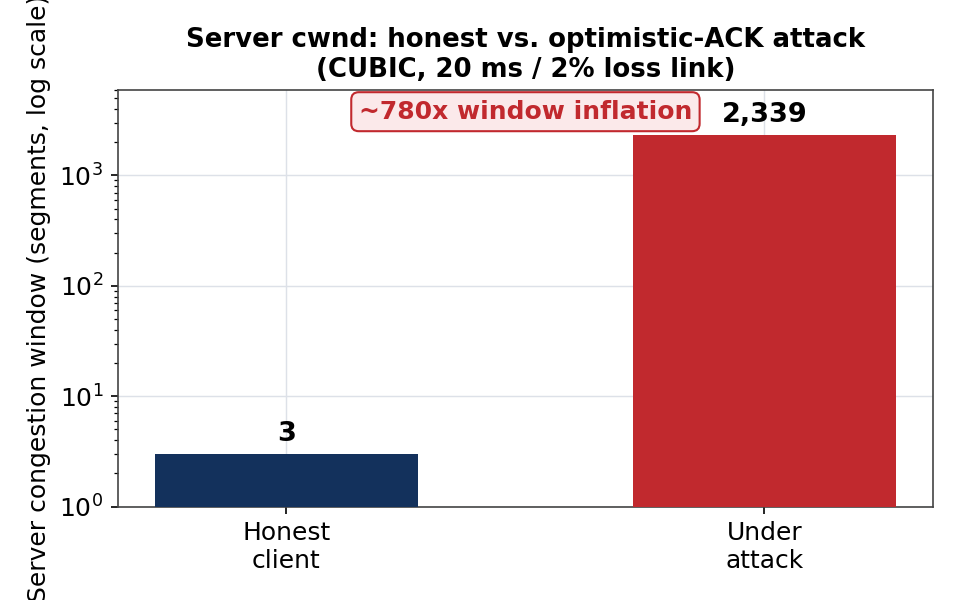
\includegraphics[width=0.49\textwidth]{figures/fig_cwnd_compare.png}\hfill
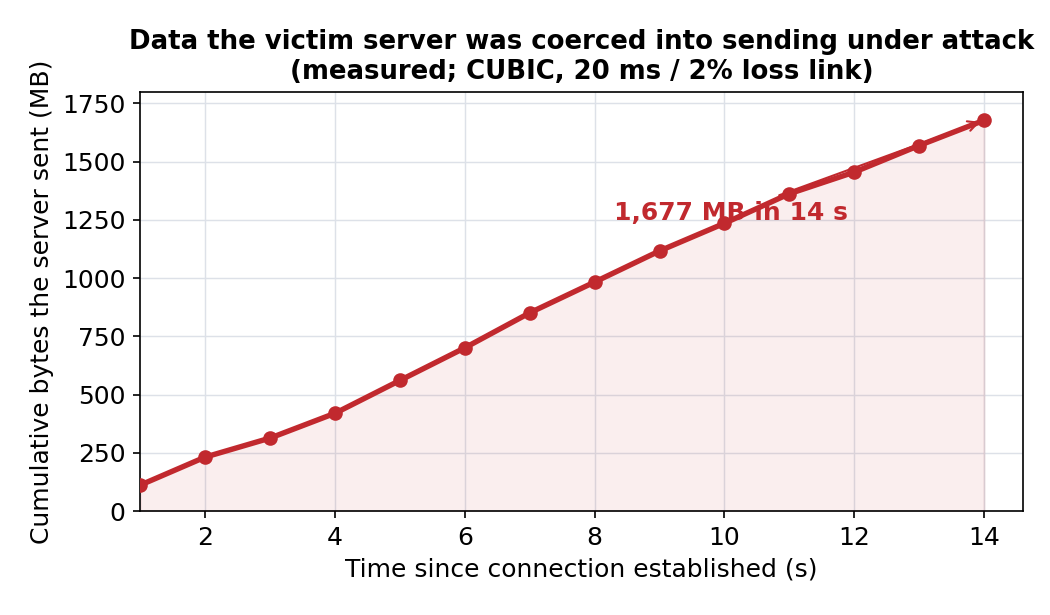
\includegraphics[width=0.49\textwidth]{figures/fig_recv_timeline.png}
\caption{\textbf{Left:} server congestion window, honest (\texttt{cwnd:3}) vs.\ attack
(\texttt{cwnd:2339}), log scale. \textbf{Right:} cumulative data the victim was coerced
into sending --- 1{,}677\,MB in 14\,s, read directly from the attacker's own counter.}
\label{fig:success}
\end{figure}

\paragraph{Why it succeeds.} The link genuinely drops 2\% of packets, and an honest CUBIC
flow respects that loss --- hence \texttt{cwnd:3} and 559 retransmissions in the control.
The attacker's optimistic ACKs \emph{conceal} that loss: the server sees only a stream of
acknowledgments arriving almost instantly, so its congestion control --- working exactly
as specified --- keeps the window wide open. The victim's \texttt{minrtt} of 0.89\,ms is
the smoking gun: no packet could physically round-trip a 20\,ms link that fast, so the
acknowledgments must be for data that had not actually completed a round trip. The attack
does not break TCP; it feeds TCP a lie that TCP has no way to detect on its own.

% ============================ 6. OBSERVED OUTPUT ============================
\section{Observed Output on Each Machine}
\label{sec:observed}

This section answers requirement~\textbf{(c)}, summarising what each node in the testbed
reports during the attack.

\begin{table}[h]
\centering\small
\begin{tabular}{@{}p{2.4cm}p{12.2cm}@{}}
\toprule
\textbf{Machine} & \textbf{Observed output during the attack} \\
\midrule
\textbf{Attacker} (172.28.0.20) & Tool reports a runaway ``received'' counter --- 1{,}677\,MB in 14\,s, thousands of tiny ACKs sent per second, and a small, self-correcting ``ack-ahead'' lead (Step~3 capture). Its actual uplink cost is negligible (only $\sim$40-byte ACKs). \\
\addlinespace
\textbf{Victim / Server} (172.28.0.10) & \texttt{ss -ti} shows \texttt{cwnd} climbing into the thousands and \texttt{minrtt} collapsing to $<$1\,ms (Step~4); \texttt{tcpdump} shows the inbound flood of zero-length ACKs; the server's egress saturates at $>$2\,Gbit/s internally --- its own bandwidth turned into the weapon. \\
\addlinespace
\textbf{Observer / honest client} (172.28.0.30) & Serves as the control: on the same link it achieves only \texttt{cwnd:3} and $\sim$1.6\,Mbit/s while honestly absorbing the 2\% loss (559 retransmits). Under a shared-link scenario this is exactly the client whose service degrades. \\
\bottomrule
\end{tabular}
\caption{Per-node observations. The asymmetry is the whole point: tiny attacker cost,
enormous victim egress.}
\end{table}

\subsection{Multi-Algorithm Characterisation}
\label{sec:matrix}
\label{sec:sweep}

To understand \emph{how far} the result generalises, we swept the attack across
congestion-control algorithm (Reno, CUBIC) $\times$ TCP timestamps $\times$ SACK, each
against a fresh honest baseline on the same link (Figure~\ref{fig:matrix}).

\begin{figure}[h]
\centering
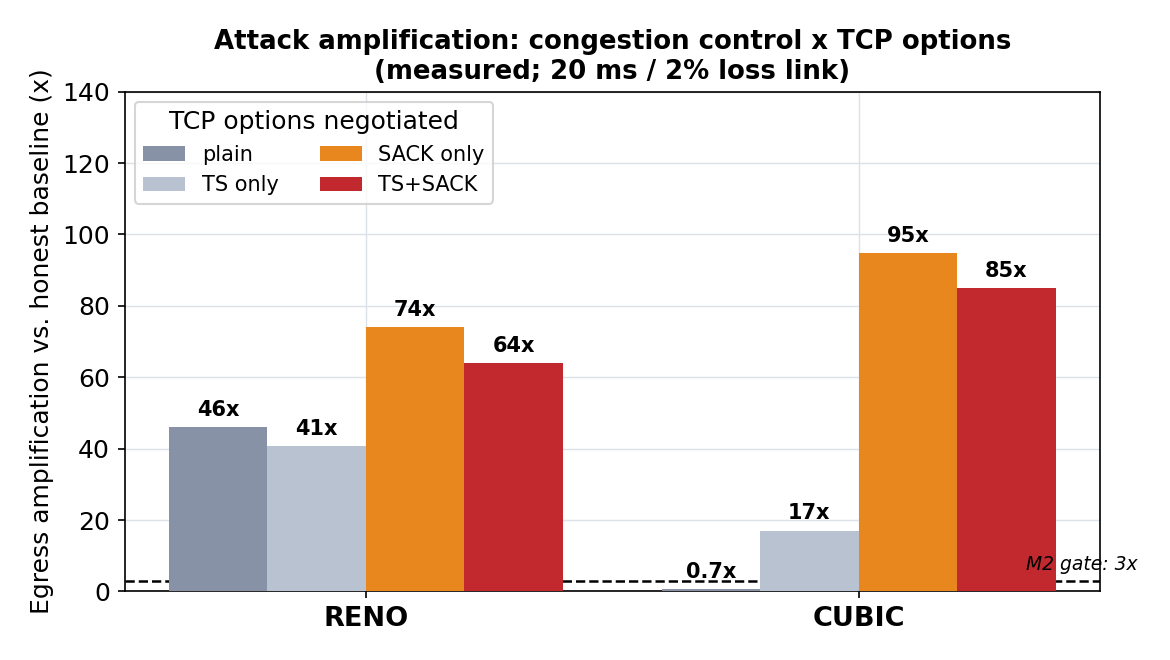
\includegraphics[width=0.86\textwidth]{figures/fig_amplification_matrix.png}
\caption{Measured egress amplification (attack $\div$ honest) across the option matrix.
Both loss-based algorithms are severely affected. The one near-miss --- CUBIC with neither
SACK nor timestamps (0.67$\times$) --- is itself a finding: without SACK the attacker's
recovery ACKs can look like duplicate ACKs and \emph{shrink} the window, so the attack can
backfire. A realistic client negotiates SACK, and there the attack is devastating
(85--95$\times$).}
\label{fig:matrix}
\end{figure}

\begin{keybox}[Finding: SACK is the reliability lever]
Loss-based congestion control (Reno, CUBIC --- the Linux default) is highly vulnerable.
\textbf{SACK, which every modern receiver negotiates, is what makes the attack reliable};
without it results are inconsistent and can even backfire. This is why our tool negotiates
SACK and timestamps by default --- it emulates a realistic modern receiver, which is the
worst case for the victim.
\end{keybox}

\begin{notebox}[On BBR and run-to-run variance]
Because \texttt{netem}'s 2\% loss is genuinely random, absolute amplification varies
between runs (we observed CUBIC ranging from $\sim$9$\times$ to $\sim$172$\times$ across
runs --- all far above any success threshold); the \emph{qualitative} result is stable.
Google's \textbf{BBR}, which paces from a bandwidth/RTT model rather than trusting every
ACK, is expected to be only \emph{boundedly} affected rather than unbounded. Docker
Desktop's kernel does not ship the \texttt{tcp\_bbr} module, so our BBR numbers are
produced by a GitHub Actions workflow on a real Linux kernel rather than locally.
\end{notebox}

% ============================ 7. DEFENSE ============================
\section{Countermeasure: The Randomly-Skipped-Segment Test}
\label{sec:defense}

This section answers requirement~\textbf{(d)}. We designed and implemented a working,
server-side defense: \textbf{Sherwood's randomly-skipped-segment test}
(\texttt{server/defense\_server.c}).

\subsection{How it works}
The defended server occasionally \emph{skips} a segment --- it advances its own send
sequence past a small gap \emph{without transmitting those bytes} --- and remembers the
hole. Then it watches the acknowledgments:

\begin{itemize}
  \item An \textbf{honest} receiver never got the skipped bytes, so its cumulative ACK
        \emph{cannot} advance past the hole; it stalls there until the server retransmits
        (which it does after a short grace period, so honest clients are never harmed).
  \item A \textbf{misbehaving optimistic} receiver is acknowledging data it never
        received, so it ACKs \emph{straight past the hole} --- which is impossible for an
        honest peer and constitutes unforgeable proof that it is lying. The server logs
        the event and resets the flow.
\end{itemize}

Because it must control its own TCP sequence numbers to leave a deliberate hole (a normal
kernel socket cannot), the defended server is itself a raw-socket server. It needs no
\texttt{netem} and no special kernel modules, so it runs anywhere Docker does. The design
deliberately resets \emph{only after positive proof} --- never merely on an out-of-window
ACK --- which avoids creating a new spoofing-based reset vulnerability.

\subsection{Before / after evidence}
With the defense enabled, the identical attack is caught on the very first skipped segment:
\begin{lstlisting}[style=term]
[defense] listening on port 5000, skip-test defense ENABLED
[defense] client 172.28.0.20:45946 connected
[defense] OPTIMISTIC ACK DETECTED: client acked 54195439, past skipped
          segment [50808239,50809699) it never received -- resetting flow
[defense] flow reset after 2500980 bytes
\end{lstlisting}

The attacker, cut off, collapses from hundreds of Mbit/s to a trickle; an honest client
on the same defended server completes normally and is never flagged:

\begin{figure}[h]
\centering
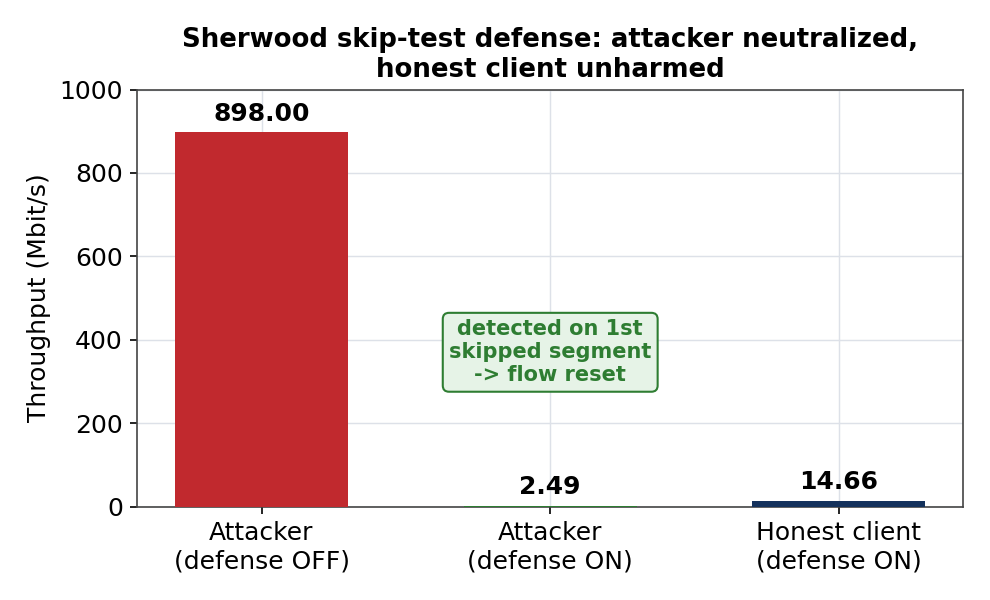
\includegraphics[width=0.66\textwidth]{figures/fig_defense.png}
\caption{Before/after the defense. The attacker's throughput drops from \textbf{898 to
2.49\,Mbit/s} once detected and reset, while an honest client transfers normally
(14.66\,MB, \textbf{zero} false detections).}
\label{fig:defense}
\end{figure}

\begin{keybox}[Defense result]
Attack detected on the 1st probe $\rightarrow$ flow reset $\rightarrow$ attacker throughput
\textbf{898\,$\rightarrow$\,2.49\,Mbit/s} ($\approx$360$\times$ reduction). Honest client:
14.66\,MB transferred, \textbf{0} false positives. The defense needs no client changes and
adds negligible overhead in the common (no-skip) case.
\end{keybox}

% ============================ 8. DASHBOARD ============================
\section{Interactive Visualisation Dashboard}

To make the attack legible in real time we built a one-command web dashboard
(Figure~\ref{fig:dashboard}). It drives the real testbed --- not a recording --- through
the Docker socket, animates packets flowing between the nodes at a rate driven by the live
measured throughput and RTT, and builds a session report table as each step runs. It
offers both a guided six-step scenario (honest baseline $\rightarrow$ attack with SACK
$\rightarrow$ without SACK $\rightarrow$ defense) and manual controls.

\begin{figure}[h]
\centering
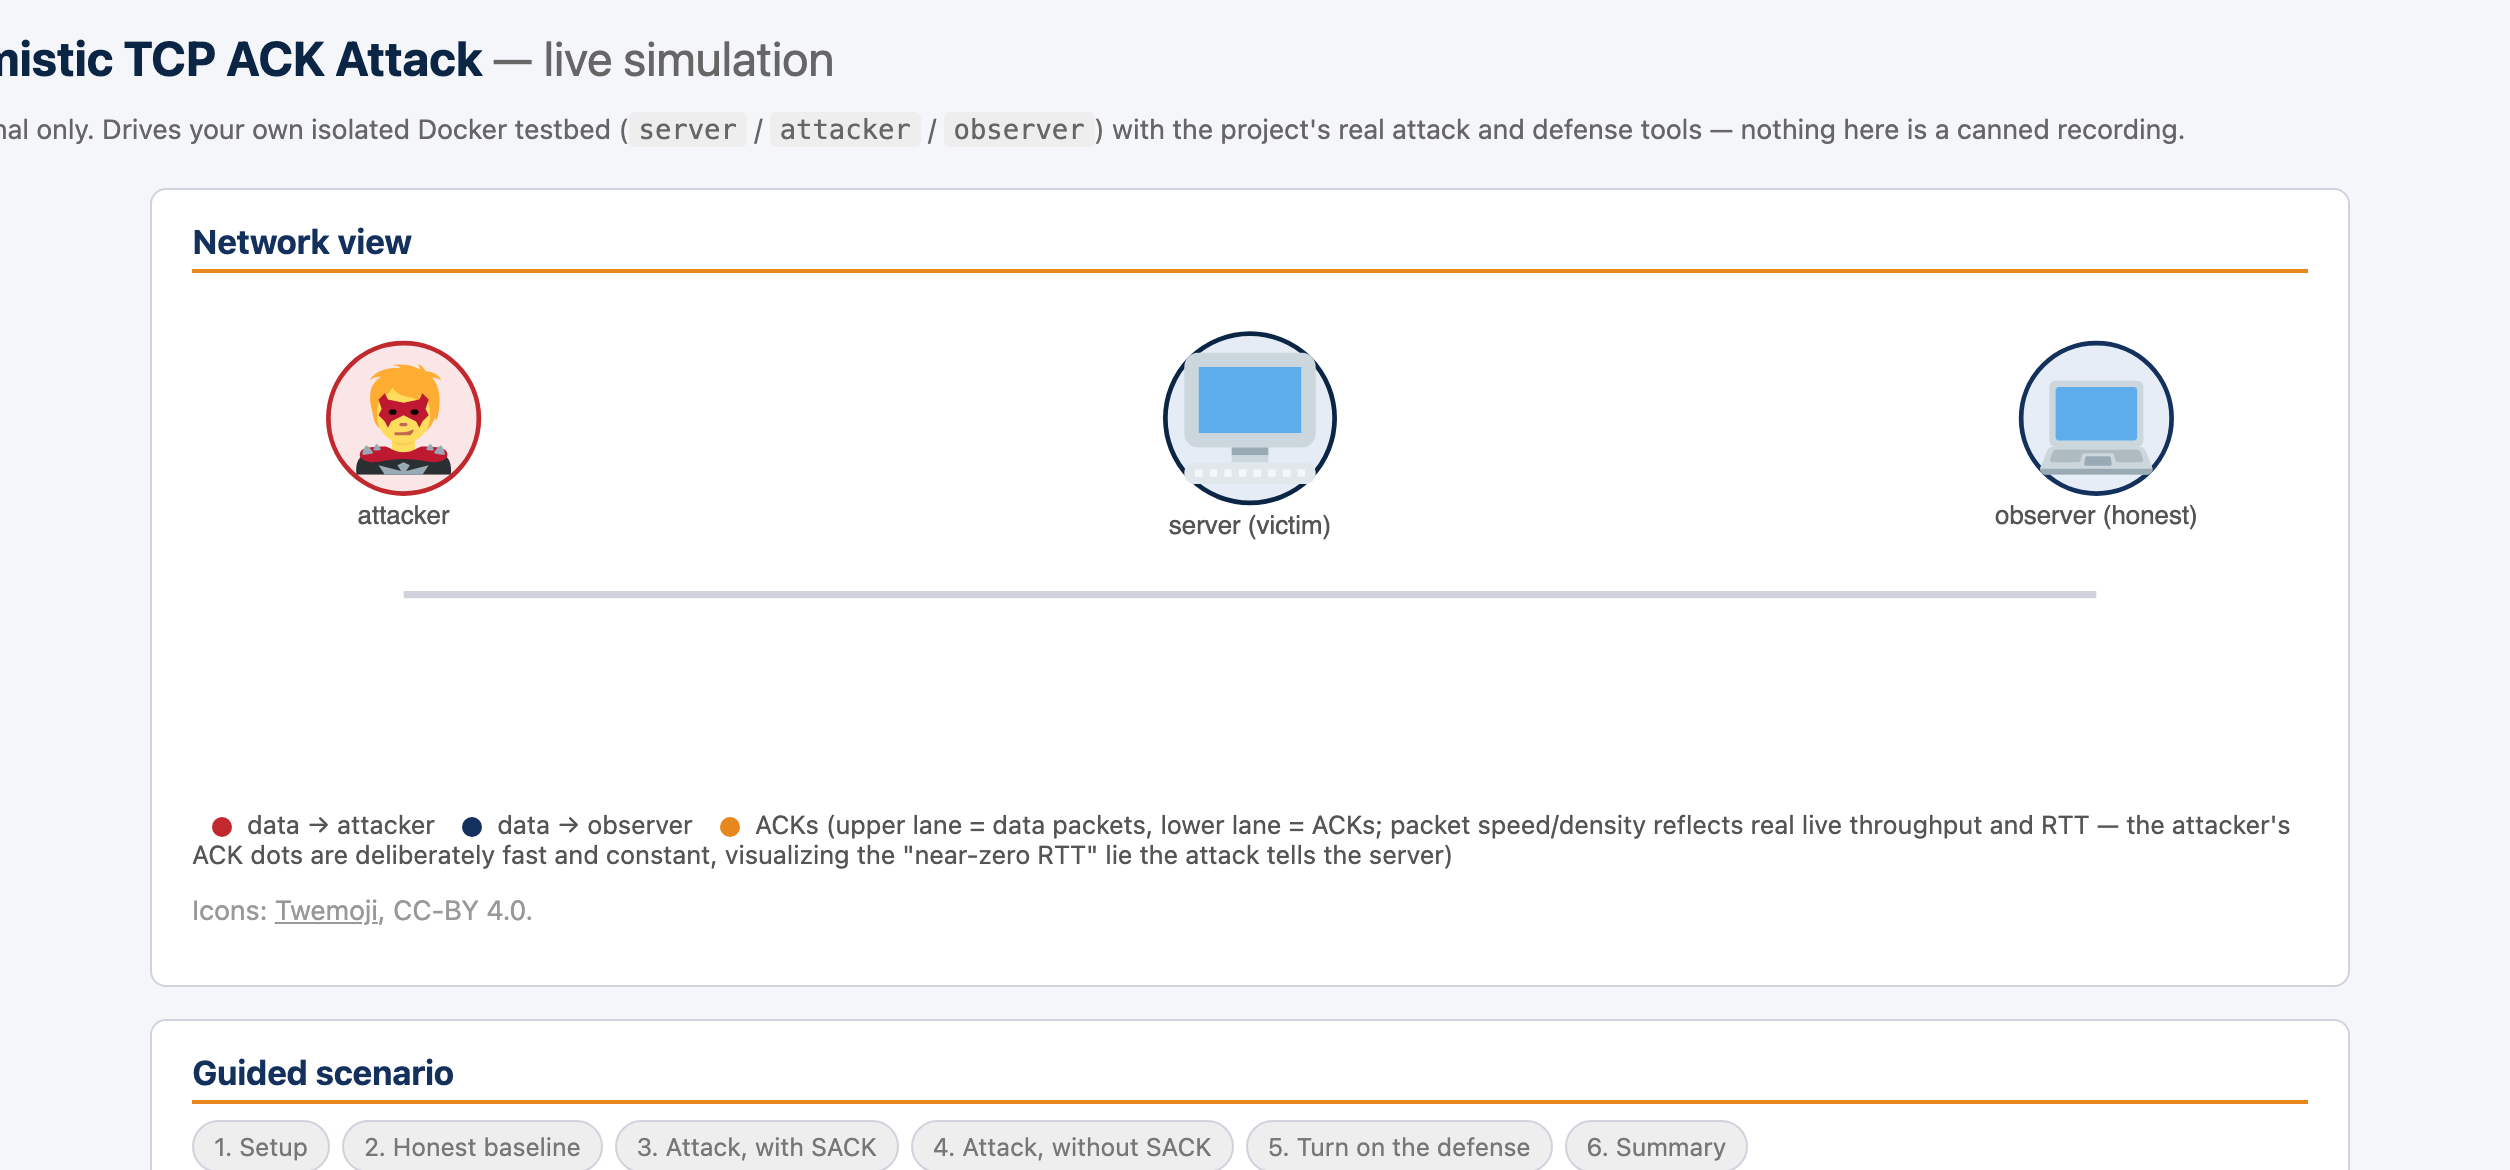
\includegraphics[width=0.92\textwidth]{figures/dashboard_networkview.png}
\caption{The live dashboard's network view. Attacker, victim server, and honest observer
are shown as nodes; during a run, animated packets flow between them at the real measured
rate, and live \texttt{cwnd}/RTT/throughput charts and a self-building results table update
beneath.}
\label{fig:dashboard}
\end{figure}

% ============================ 9. REPRODUCIBILITY ============================
\section{Reproducibility}

The whole project comes up with one command, and every milestone gate can be re-run
end-to-end:
\begin{lstlisting}[style=codebox]
docker compose up -d --build      # server + attacker + observer + dashboard
./scripts/run_all_gates.sh        # re-runs every milestone gate; prints ALL GATES PASSED
\end{lstlisting}
On our final audit this reported \texttt{ALL GATES PASSED} (M0 baseline, M1 cubic/reno,
M2 attack, M3 sweep, M4 defense; BBR correctly skipped for the documented kernel reason).
Attack timing and sequence numbers are seedable (\texttt{--seed} / \texttt{ATTACK\_SEED} /
\texttt{DEFENSE\_SEED}) for exact repeatability; seed determinism was verified (identical
seed $\rightarrow$ identical initial sequence number).

% ============================ 10. LIMITATIONS ============================
\section{Limitations}
\textbf{BBR requires a real kernel.} Our local test host (Docker Desktop's LinuxKit
kernel) does not ship the \texttt{tcp\_bbr} module, so only Reno and CUBIC could be
measured locally. The attack tool, the streaming server, and the harness all support BBR
already; the BBR numbers are therefore produced by a GitHub Actions workflow running on a
real Linux kernel (\texttt{ubuntu-latest}) rather than on our own machine. Per the
aBBRate study~\cite{abbrate}, BBR --- which paces from a bandwidth/RTT model rather than
trusting every ACK --- is expected to be only \emph{boundedly} affected by this attack,
in contrast to the unbounded window inflation seen on the loss-based algorithms we
measured.

% ============================ 11. CONCLUSION ============================
\section{Conclusion}
We built the optimistic TCP ACK attack from scratch, demonstrated it decisively against a
CUBIC streaming server ($\approx$780$\times$ window inflation, up to $\sim$95$\times$
egress amplification), explained precisely why it succeeds (loss concealment defeats the
only brake loss-based congestion control has), characterised its reach across Reno/CUBIC
and the SACK/timestamps options, and implemented a working defense that detects and
neutralises it on the first probe without harming honest clients. The attack is not a bug
to be patched but a consequence of TCP trusting its receivers; the defense works by
manufacturing a situation in which a lying receiver must reveal itself.

% ============================ REFERENCES ============================
\begin{thebibliography}{9}
\small
\bibitem{savage} S.~Savage, N.~Cardwell, D.~Wetherall, T.~Anderson.
``TCP Congestion Control with a Misbehaving Receiver.''
\textit{ACM SIGCOMM CCR}, 29(5), 1999.
\bibitem{sherwood} R.~Sherwood, B.~Bhattacharjee, R.~Braud.
``Misbehaving TCP Receivers Can Cause Internet-Wide Congestion Collapse.''
\textit{ACM CCS}, 2005.
\bibitem{abbrate} R.~Peterson, S.~Jero, E.~Hoque, D.~Choffnes, C.~Nita-Rotaru.
``aBBRate: Automating BBR Attack Exploration Using a Model-Based Approach.''
\textit{RAID}, 2020.
\bibitem{rfc5681} M.~Allman, V.~Paxson, E.~Blanton. ``TCP Congestion Control.''
RFC~5681, IETF, 2009.
\end{thebibliography}

\end{document}
